\documentclass[12pt]{article}

\usepackage{graphicx}

\begin{document}
\title{TP 1 Deliverable}
\author{Ryan Bao (ryanbao)}
\date{11/28/2020}
\maketitle
\pagenumbering{roman}
\tableofcontents
\listoffigures
\newpage
\pagenumbering{arabic}
\section{Project Proposal}
\subsection{Project Description}
    My term project is called 'The Box Game' and is an open world game
with random, seed-based map generation. The game will also include 
a grid-based crafting system, similar to that of Minecraft, but also
with an RNG based system for the 'quality' of the items. The game 
movement will be based around the WASD keys, with side scrolling chunks
when you get to the edge of the screen. Combat systems will be based 
around mouseclicks, with a combination of ranged and melee attacks. 
The enemies will pathfind based on slight modifications of the astar 
algorithm. 

\begin{figure}[h]
    \centering
    
\includegraphics[width = 3cm]{char.PNG}
    \caption{Example character design}
\end{figure}

\subsection{Competitive Analysis}
    The closest games to this term project are Genshin Impact, a recently
released RPG game, and Minecraft, a relatiely old open-world survival 
game. This game will take many of the element of Genshin Impact, such 
as a similar combat system and, if time permits, a similar art style, 
although it will be a simplified, top-down, 2 dimensional version of 
the game, similar to the Pokemon games. This game will also incorporate 
an RNG-based system for crafting, similar to Genshin Impact cooking
mechanics. 

This game will also be similar to Minecraft in the terrain modification, 
crafting system, and random seed-based generation. This game uses a heavily 
simplified version of Minecraft random chunk-based generation, where
each chunk is generated separately and then placed into a 2-dimensional
list that represents the map. Similarly, the crafting system will be 
grid-based, similar to that of Minecraft, although the exact details
of such a system have yet to be hashed out fully. The game also incorporates
somewhat modifiable terrain, with obstacle destruction, and, time permitting,
a limited building system, similarly to that of Minecraft.

\subsection{Structural Plan}
The majority of the structure of the project has already been created. 
The code will be organized into different code documents, based on 
reasonable categories. For example, one such category is enemyCode.py, 
which includes the enemy class, an enemy movement function that can 
be placed into timerFired in the main code, as well as enemy generation
functions that help map generation, as defined in mapCode. The rest of
the project will be organized similarly. Most of the necessary objects
have been created already. The last class before MVP would be a class
for crafting recipes. The code is designed to have as little as possible
in the main code class. Ideally, only the functions that are required for
cmu\_112\_graphics, such as redrawAll, timerFired, appStarted, and such
will be included, with all other functions on separate documents to 
promote readibility.

\subsection{Algorithmic Plan}
The central algorithmic complexity of the project will be in the enemy
movement algorithm, which will be based on the A* pathfinding algorithm.
In a simplified version of the algorithm, a list of moves that are an 
specified distance away from the enemy and separated by a specified angle
theta will be evaluated, and the optimal move will be selected from those
moves based on the distance traveled by the enemy, as well as the distance 
between the enemy and the player character. For ranged enemies, a 
slightly modified version of the algorithm will be used, where the 
enemy selects the move that keeps them within optimal distance with the
player character while also looking for a clear line-of-sight between
the enemy and the player character. 

Another core algorithm of the project will be the crafting algorithm.
Although the details of this algorithm have yet to be determined, 
crafting recipes will probably be stored in a 2-dimensional list of 
dimensions 3x3, with None being used to fill the empty spaces. Then, the player, 
in the crafting UI, the player will have the option of filling each of 
the spaces with an item of their choice. If the grid fits one of the
defined crafting recipes, the completed item will show up in the UI
and the player will have the option of claiming it. If the player
does choose to claim it, an RNG system will be used to determine the quality
of the item. 

\subsection{Timeline Plan}
At the writing of this document, the majority of the combat system has 
been determined. The only components left are item drops when an obstacle
or enemy is destroyed, as well as a few minor bugs in the A* algorithm.
Therefore, the majority of next week will be devoted to updating the 
graphics of the program, as well as determining a crafting system. 

\subsection{Version control plan}
The code for this project will be backed up using Github. Each version
of code will be pushed to main, and then a new, numerical branch will
be created to specifiy the version of the code. 

\begin{figure}[h]
    \centering
    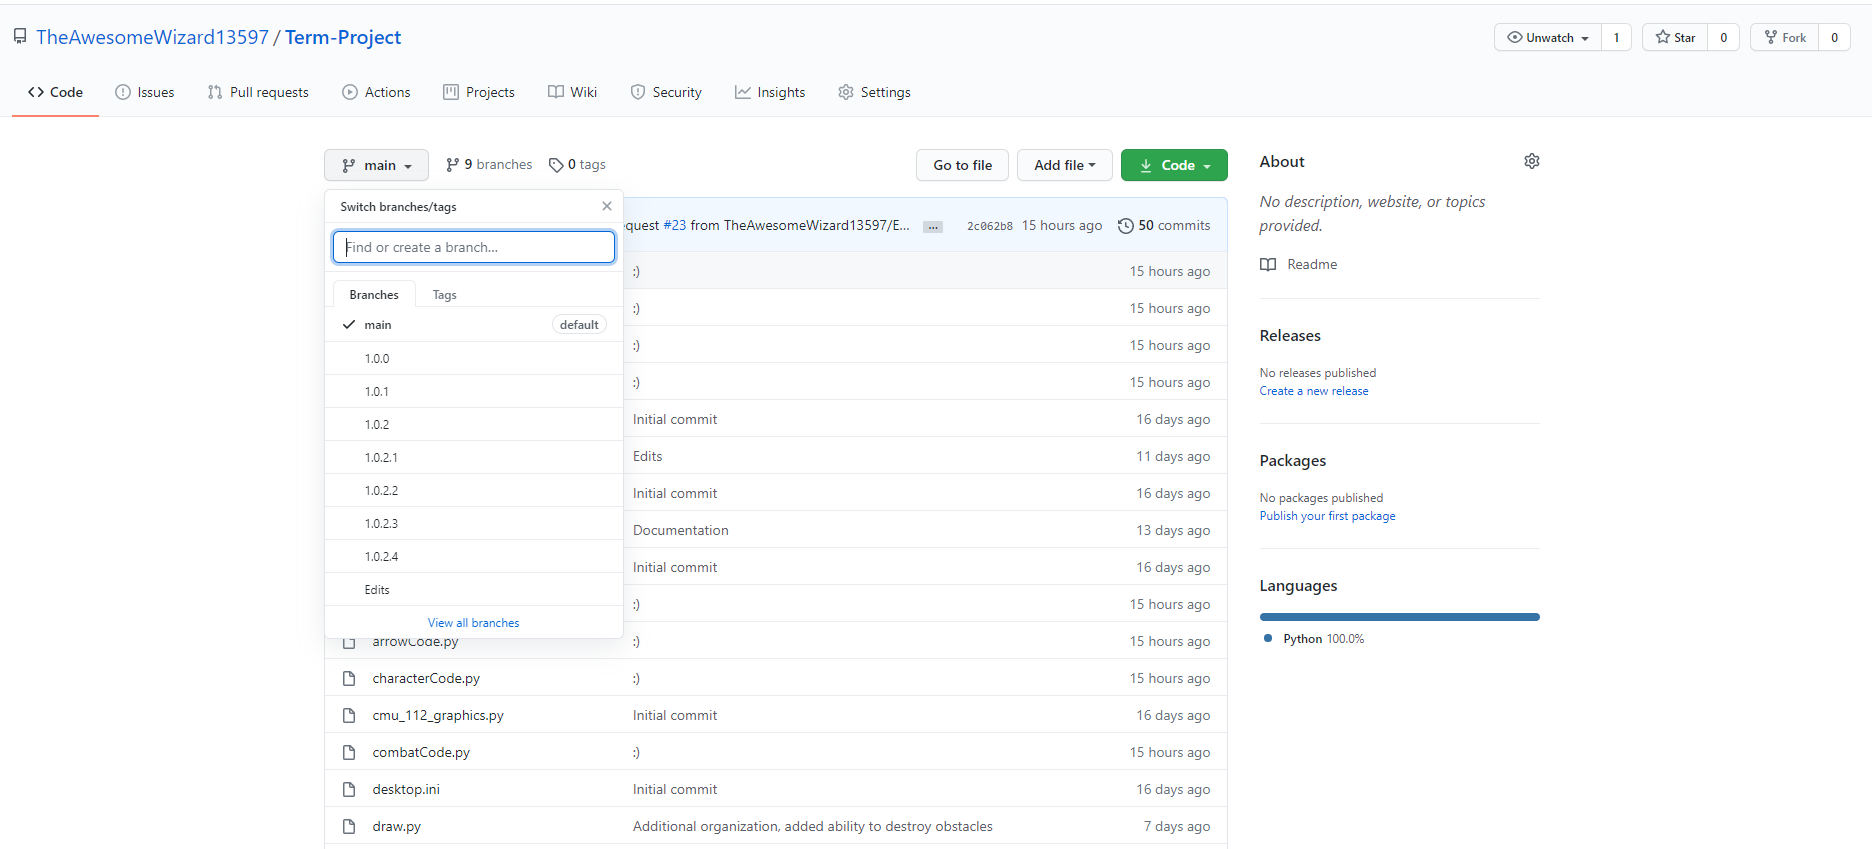
\includegraphics[width = 10cm]{Capture}
    \caption{Image of Github page with version control}
\end{figure}

\subsection{Module List}
The code for this project will include the pandas module, confirmed in 
my tech demo. It also includes a small function from numpy, which will
be superseded in a later version. 
\newpage
\section{Storyboard}
\begin{figure}[h]
    \centering
    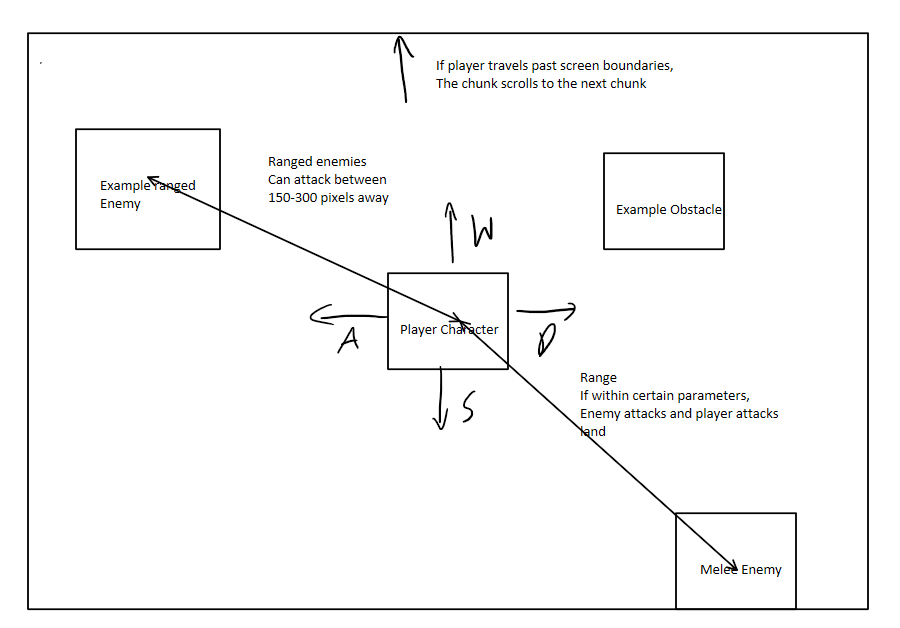
\includegraphics[width = 10cm]{Storyboard0.PNG}
    \caption{Storyboard showing basic enemy and player interactions}
\end{figure}
\begin{figure}[b]
    \centering
    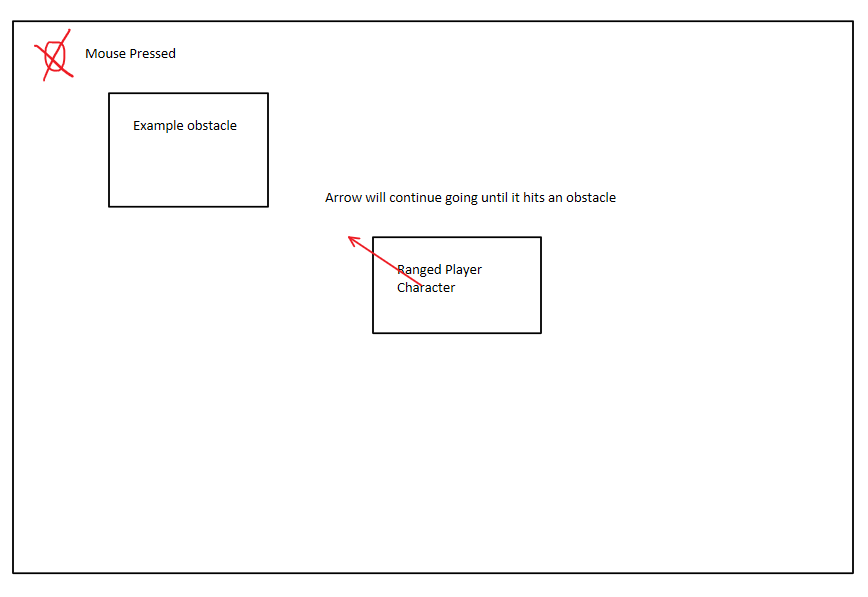
\includegraphics[width = 10cm]{Storyboard1.PNG}
    \caption{Storyboard showing player ranged attack interactions}
\end{figure}
\begin{figure}[h]
    \centering
    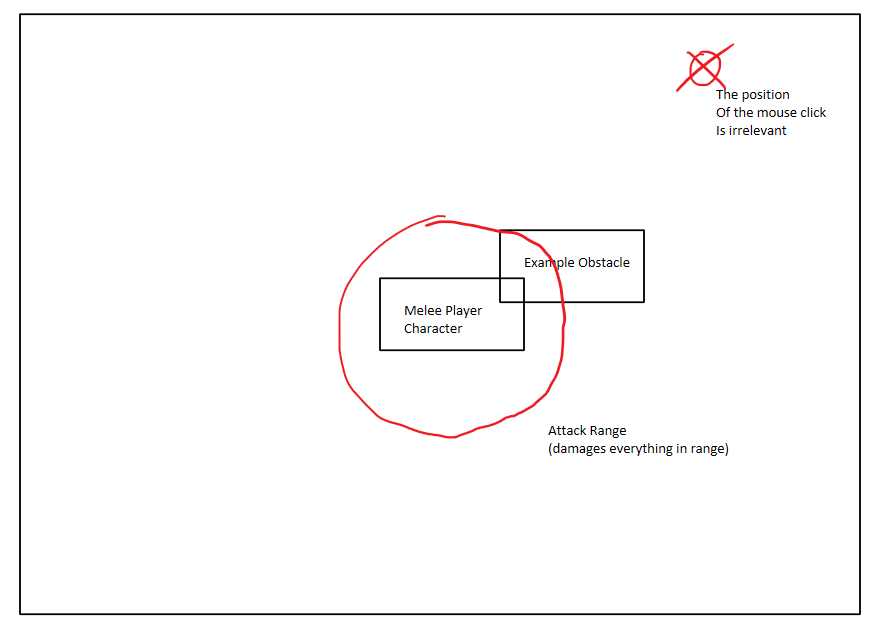
\includegraphics[width = 10cm]{Storyboard2.PNG}
    \caption{Storyboard showing player melee attack interactions}
\end{figure}
\begin{figure}[h]
    \centering
    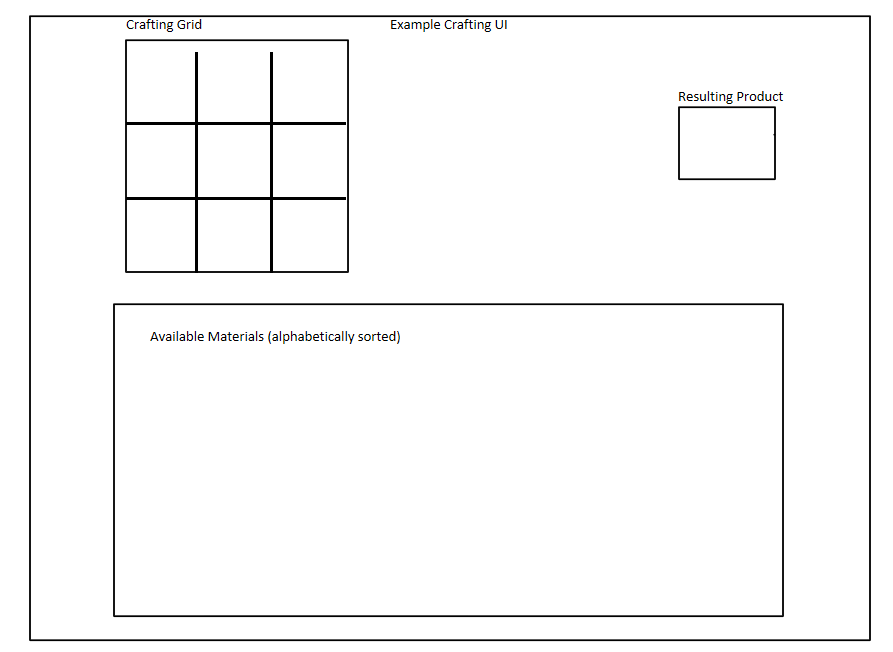
\includegraphics[width = 10cm]{Storyboard3.PNG}
    \caption{Storyboard showing planned crafting interface}
\end{figure}
\begin{figure}[h]
    \centering
    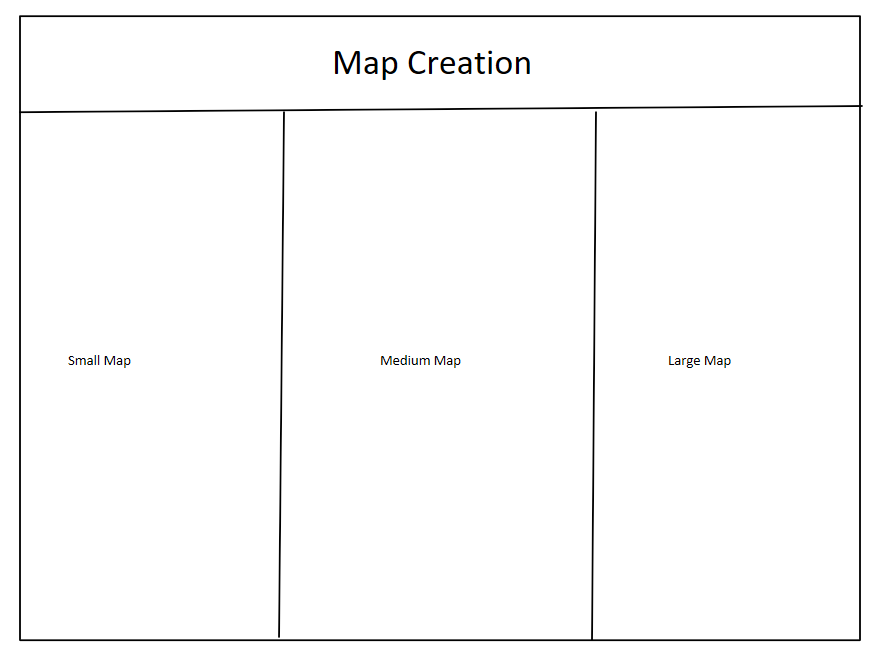
\includegraphics[width = 10cm]{Storyboard4.PNG}
    \caption{Storyboard showing planned map creation interface}
\end{figure}
\begin{figure}[h]
    \centering
    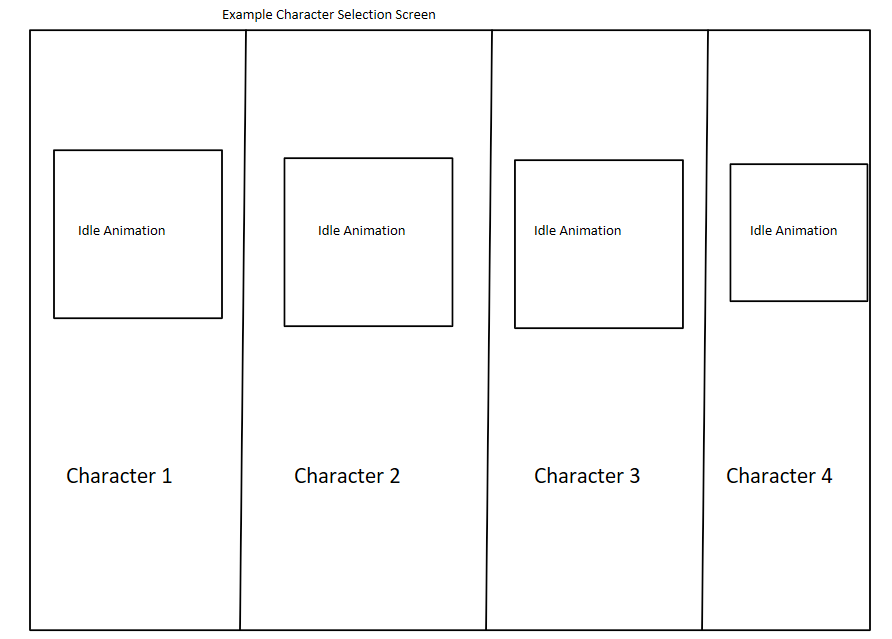
\includegraphics[width = 10cm]{Storyboard5.PNG}
    \caption{Storyboard showing planned character selection screen}
\end{figure}
\end{document}